% paper.tex  —  v2
% Agency Decomposition via Path Diversity:
% SCC-Condensation Metrics for Goal-Directed Systems
%
% v2 changes (from hostile referee review):
%   F1  EA = AI × PDI reframed as Definition (not Theorem); orthogonality
%       claim removed; multiplicative form motivated by dimensional independence
%   F2  No Artificial Inflation proof rewritten: path distinctness defined
%       via SCC-node sequences in Ĝ; overcounting argument made precise
%   F3  Type error fixed: |M|/|R| throughout; initial-state path convention
%       stated explicitly
%   F4  §7.1 relabelled "Reference Exemplar Survey"; table of 9 systems added;
%       "naturalistic" language removed
%   F5  Theorem 3 (Upper Bound) removed; replaced by Proposition (Cyclic Grid)
%       with closed-form PDI and proof
%   F6  Cyclic Thrashing proof rewritten: pigeonhole argument for periodicity;
%       PI=0 + finite state-space; "sink SCC" condition made explicit
%   M1  Merge Stability Criterion: circularity removed; restated for R, not M
%   M4  Theorem 4 (Lower Bound) removed; absorbed into Proposition
%
% Compile: pdflatex paper && bibtex paper && pdflatex paper && pdflatex paper

\documentclass[11pt,letterpaper]{article}

\usepackage[margin=1.15in]{geometry}
\usepackage{amsmath,amssymb,amsthm}
\usepackage{graphicx}
\usepackage{booktabs}
\usepackage{hyperref}
\usepackage{xcolor}
\usepackage[numbers,sort&compress]{natbib}
\PassOptionsToPackage{hyphens}{url}  % allow URL line breaks at hyphens/slashes

% ── theorem environments ──────────────────────────────────────────────────────
\theoremstyle{plain}
\newtheorem{theorem}{Theorem}
\newtheorem{lemma}[theorem]{Lemma}
\newtheorem{proposition}[theorem]{Proposition}
\newtheorem{corollary}[theorem]{Corollary}
\theoremstyle{definition}
\newtheorem{definition}[theorem]{Definition}
\theoremstyle{remark}
\newtheorem{remark}[theorem]{Remark}

% ── macros ────────────────────────────────────────────────────────────────────
\newcommand{\PDI}{\mathrm{PDI}}
\newcommand{\AI}{\mathrm{AI}}
\newcommand{\PI}{\mathrm{PI}}
\newcommand{\EA}{\mathrm{EA}}
\newcommand{\GD}{\mathrm{GD}}
\newcommand{\CE}{\mathrm{CE}}
% \textup{} forces upright shape so \textsc works in italic theorem bodies
\newcommand{\OK}{\textup{\textsc{ok}}}
\newcommand{\PB}{\textup{\textsc{pb}}}
\newcommand{\IV}{\textup{\textsc{iv}}}
\newcommand{\OD}{\textup{\textsc{ood}}}
\newcommand{\carrier}{\mathcal{F}}
\newcommand{\jn}{\vee}  % join in failure algebra
\newcommand{\gens}{\mathcal{G}}
\newcommand{\Ghat}{\hat{G}}

\hypersetup{
  colorlinks=true, linkcolor=black, citecolor=black, urlcolor=blue,
  pdftitle={Agency Decomposition via Path Diversity v2},
  pdfauthor={QA Research}
}
\setlength{\emergencystretch}{3em}  % last-resort stretch to avoid bibliography URL overfull

% ─────────────────────────────────────────────────────────────────────────────
\begin{document}

\title{\textbf{Agency Decomposition via Path Diversity:}\\
       SCC-Condensation Metrics for Goal-Directed Systems}

\author{QA Research}
\date{March 2026 \quad|\quad
      arXiv preprint (v2) \quad|\quad
      \href{https://github.com/1r0nw1ll/quantum-arithmetic-research}{%
        \texttt{github.com/1r0nw1ll/quantum-arithmetic-research}}}

\maketitle

% ─────────────────────────────────────────────────────────────────────────────
\begin{abstract}
We introduce the \emph{Path Diversity Index} ($\PDI$), a structural metric
quantifying counterfactual route richness in goal-directed systems.
$\PDI = |M|/|R|$ counts the fraction of reachable states with $\geq 2$
distinct directed paths from the initial state set, where paths are counted
as distinct sequences of SCC nodes in the condensation DAG $\Ghat$ of the
system's generator graph.
Together with the Plasticity Index ($\PI$), $\PDI$ defines four behavioral
regimes --- \emph{Frozen}, \emph{Linear Explorer},
\emph{Stuck-Loop Thrashing}, and \emph{Flexible Planner} ---
via the \emph{Effective Agency} definition $\EA = \AI \times \PDI$.
We prove three structural results: the SCC Saturation Lemma,
No Artificial Inflation Theorem (cycles inflate path counts only
on the uncondensed graph, not on $\Ghat$), and the Cyclic
Thrashing Theorem (finite deterministic systems with $\PI = 0$
and a sink cycle exhibit thrashing).
We give a closed-form $\PDI$ for the $A$-arm cyclic cross-link grid
and show that $\PDI > 0.5$ iff $A(D-1) > (1+AD)/2$.
We connect $\PDI$ to the QA failure algebra via the
\emph{PDI--Obstruction Bridge}: generator failure tags
determine whether obstructions are topology-preserving (Type~III)
or route-reducing (Type~II).
Nine synthetic reference exemplars all fall below $\PDI = 0.5$
(range $0.425$--$0.475$), confirming that no deliberate merge engineering
is present in standard curated competency benchmarks.
A constructive FLEXIBLE PLANNER ($\PDI = 0.800$, $\PI = 0.750$) is built
from an all-$\OK$-tagged grid, and a controlled perturbation establishes
$\PDI(k) = 0.800 - 0.200k$ with regime collapse at $k=2$.
\end{abstract}

% ─────────────────────────────────────────────────────────────────────────────
\section{Introduction}

What makes an agent \emph{flexibly} goal-directed rather than merely
\emph{competent}?
Existing frameworks for system competency --- including Levin's
control-theoretic account of biological cognition
\cite{levin2019regenerative,levin2022technological} and
Fields \& Levin's competency metric suite \cite{fields2022competency} ---
characterize the \emph{size} of a system's reachable state space (Agency
Index, $\AI = |R|/T$) and the \emph{speed} at which it adapts to perturbation
(Plasticity Index, $\PI = \delta_R/\delta_P$).
Neither metric captures a third structural property:
whether the system has multiple independent routes to its goals,
the property that distinguishes a system that can
\emph{recover from generator failure} from one that cannot.

We introduce the \emph{Path Diversity Index} ($\PDI$) to fill this gap.
$\PDI$ measures the fraction of reachable states accessible via at least
two distinct directed paths in the SCC-condensation DAG $\Ghat$.
Informally: $\PDI$ asks whether the system's reachability structure is a
tree (single route per state) or a DAG with merging branches.

The main contributions of this paper are:
\begin{enumerate}
  \item \textbf{Definition and algorithm} (\S\ref{sec:definition}):
    $\PDI$ via Tarjan SCC-condensation \cite{tarjan1972depth,cormen2022introduction},
    complexity $O(|V|+|E|)$, with explicit path-distinctness convention.
  \item \textbf{Structural results} (\S\ref{sec:theory}):
    SCC Saturation Lemma, No Artificial Inflation Theorem,
    Cyclic Grid Proposition, and Cyclic Thrashing Theorem.
  \item \textbf{Regime classification} (\S\ref{sec:regimes}):
    four-quadrant $(\PI, \PDI)$ map; Effective Agency $\EA = \AI \times \PDI$
    defined as a product of independent structural dimensions.
  \item \textbf{Obstruction algebra bridge} (\S\ref{sec:bridge}):
    failure tags $\to$ obstruction types $\to$ $\PDI$ sensitivity.
  \item \textbf{Experiments} (\S\ref{sec:experiments}):
    nine synthetic reference exemplars; constructive existence proof;
    controlled fragility experiment.
\end{enumerate}

% ─────────────────────────────────────────────────────────────────────────────
\section{Background and Setup}
\label{sec:setup}

\paragraph{Generator graph.}
A goal-directed system is modelled as a directed graph $G = (V, E, I, F)$
where $V$ is the state space, $E$ contains a directed edge $(u,v,g)$ whenever
generator $g \in \gens$ maps state $u$ to state $v$,
$I \subseteq V$ is the set of initial states, and $F \subseteq V$ is the set
of goal (attractor) states.
We write $R \subseteq V$ for the set of states reachable from $I$ under any
generator sequence, $|R|$ for its cardinality,
and $T = |V|$ for the total state count.

\paragraph{SCC-condensation DAG.}
The SCC-condensation $\Ghat$ of $G$ is computed via Tarjan's algorithm
\cite{tarjan1972depth}: each strongly connected component (SCC) is collapsed
to a single node, and all inter-SCC edges are retained.
$\Ghat$ is a DAG.
A \emph{trivial SCC} contains a single state with no self-loop;
a \emph{non-trivial SCC} contains a directed cycle.

\paragraph{Existing metrics.}
The QA Competency Detection Framework \cite{QAFamily26Cert} defines:
\[
  \AI = |R|/T, \quad
  \PI = \delta_R/\delta_P, \quad
  \GD = |F|/T, \quad
  \CE = -\textstyle\sum_g p(g)\ln p(g).
\]
$\AI$ measures control-region extent; $\PI$ measures temporal plasticity
(sensitivity of $|R|$ to perturbation); $\GD$ measures goal concentration;
$\CE$ measures generator diversity \cite{shannon1948mathematical}.

% ─────────────────────────────────────────────────────────────────────────────
\section{Path Diversity Index}
\label{sec:definition}

\paragraph{Path distinctness convention.}
A \emph{directed path} from $s \in I$ to $v \in R$ is a sequence of SCC
nodes in $\Ghat$ starting at the SCC containing $s$ and ending at the
SCC containing $v$.
Two paths $\pi_1, \pi_2$ are \emph{distinct} iff they differ as
sequences of SCC nodes.
Paths that traverse the same SCC sequence but differ by intra-SCC routing
in $G$ are treated as a single path.
This convention ensures that cyclic detours within an SCC do not
artificially inflate the path count (see Theorem~\ref{thm:no_inflate}).

\begin{definition}[Multi-path state]
\label{def:mps}
  State $v \in R \setminus I$ is a \emph{multi-path state} if there
  exist at least two distinct directed paths from $I$ to $v$ in $\Ghat$.
  States in $I$ are assigned path-count~$1$ by convention (they are
  reachable via the empty path; they are multi-path only if
  additionally reachable via a non-trivial generator sequence,
  which reduces to the general case).
  Let $M \subseteq R$ denote the set of all multi-path states.
\end{definition}

\begin{definition}[Path Diversity Index]
\label{def:pdi}
  \[
    \PDI(G) \;=\; \frac{|M|}{|R|}.
  \]
  $\PDI = 0$ iff no reachable state (outside $I$) has two independent routes;
  $\PDI = 1$ iff every reachable state is multi-path.
\end{definition}

\paragraph{Computation.}
Run Tarjan's SCC algorithm to obtain $\Ghat$ in $O(|V|+|E|)$.
Assign initial path-counts: $\mathrm{cnt}[s] \leftarrow 1$ for each $s \in I$;
$\mathrm{cnt}[v] \leftarrow 0$ for all $v \in R \setminus I$.
Process nodes of $\Ghat$ in reverse topological order:
\begin{itemize}
  \item For every trivial SCC node $C = \{v\}$:
    $\mathrm{cnt}[v] \leftarrow \min\bigl(\sum_{u \to v \in \Ghat} \mathrm{cnt}[u],\, 2\bigr)$.
  \item For every non-trivial SCC node $C$ (after updating $C$'s count
    from its condensation predecessors): if $\mathrm{cnt}[C] \geq 2$,
    saturate all original states in $C$ to count~$2$.
\end{itemize}
$|M| = |\{v \in R : \mathrm{cnt}[v] \geq 2\}|$.
Total complexity: $O(|V|+|E|)$.

% ─────────────────────────────────────────────────────────────────────────────
\section{Structural Results}
\label{sec:theory}

\begin{lemma}[SCC Saturation]
  \label{lem:scc_sat}
  Let $C$ be a non-trivial SCC.
  If any state in $C$ is reachable via $\geq 2$ distinct paths from $I$
  in $\Ghat$, then every state in $C$ is reachable via $\geq 2$ distinct
  paths from $I$.
\end{lemma}
\begin{proof}
  Let $v \in C$ be reachable via distinct paths $\pi_1 \neq \pi_2$ in $\Ghat$.
  For any $w \in C$, there exists an intra-SCC path $\rho: v \leadsto w$ in $G$.
  In $\Ghat$, this corresponds to remaining at the node $C$.
  Consider the two condensation paths $\pi_1 \cdot (C \text{ self-step}) \cdots$
  and $\pi_2 \cdot (C \text{ self-step}) \cdots$: since $\pi_1 \neq \pi_2$
  they differ in their SCC-prefix, hence they are distinct paths to $w$.
  (Formally: a path to $w$ is the SCC-sequence ending at $C$, which
  records how $C$ was entered; $\pi_1$ and $\pi_2$ enter $C$ via different
  SCC-sequences by assumption, so the two paths to $w$ inherit distinct
  SCC-prefixes.)
\end{proof}

\begin{theorem}[No Artificial Inflation]
  \label{thm:no_inflate}
  The path-counting algorithm of \S\ref{sec:definition} computes $|M|$
  exactly under the distinctness convention (Definition~\ref{def:mps}).
  Any algorithm that counts paths directly on $G$ without condensation
  can overcount $|M|$.
\end{theorem}
\begin{proof}
  Under the convention, two paths are identical iff they traverse the same
  sequence of SCC nodes in $\Ghat$.
  The algorithm propagates counts in topological order of $\Ghat$, capping
  at~$2$; it counts exactly the number of distinct SCC-node sequences from
  $I$ to each $v$, which matches Definition~\ref{def:mps}.

  \emph{Overcounting on $G$:}
  Consider a non-trivial SCC $C$ with two back-edges $e_1, e_2$ (both
  intra-SCC).
  A path in $G$ that uses $e_1$ and a path that uses $e_2$ may differ as
  edge sequences in $G$ while mapping to the \emph{same} SCC-node sequence
  in $\Ghat$ (both stay within $C$).
  An algorithm that counts paths in $G$ without condensation treats these
  as distinct, inflating the count.
  The condensation eliminates this inflation by definition. \qed
\end{proof}

\begin{proposition}[Cyclic Grid PDI]
  \label{prop:grid_pdi}
  Let $G_{A,D}$ be the \emph{$A$-arm depth-$D$ cyclic cross-link grid}:
  one apex state $s_0$; arm states $\mathrm{arm}_{k,d}$ for $k \in \{0,\ldots,A{-}1\}$,
  $d \in \{1,\ldots,D\}$; generators
  \[
    \texttt{adv}_k: \mathrm{arm}_{k,d} \to \mathrm{arm}_{k,d+1}
    \quad\text{and}\quad
    \texttt{cl}_k: \mathrm{arm}_{k,d} \to \mathrm{arm}_{(k+1)\%A,\,d+1},
  \]
  all $\tau = \OK$.
  Then:
  \[
    |R| = 1 + AD, \qquad |M| = A(D-1), \qquad
    \PDI(G_{A,D}) = \frac{A(D-1)}{1+AD}.
  \]
  In particular, $\PDI > 1/2$ iff $2A(D-1) > 1 + AD$,
  i.e.\ $AD - 2A > 1$, satisfied for all $A \geq 2$, $D \geq 3$
  (and all $A \geq 3$, $D \geq 2$).
\end{proposition}
\begin{proof}
  $G_{A,D}$ is acyclic (depth strictly increases), so $\Ghat = G_{A,D}$.
  The apex $s_0 \in I$ has path-count~$1$.
  Each $\mathrm{arm}_{k,1}$ is reachable only from $s_0$ via $\texttt{adv}_k$:
  count~$1$, not in $M$.
  For $d \geq 2$: $\mathrm{arm}_{k,d}$ has two distinct predecessors in
  $\Ghat$: $\mathrm{arm}_{k,d-1}$ via $\texttt{adv}_k$ (count $\geq 1$)
  and $\mathrm{arm}_{(k-1)\%A,\,d-1}$ via $\texttt{cl}_{(k-1)\%A}$
  (count $\geq 1$); these are distinct SCC-node sequences since they pass
  through different arm states at depth $d-1$.
  Thus $\mathrm{cnt}[\mathrm{arm}_{k,d}] = \min(1+1, 2) = 2$ for all $d \geq 2$:
  all $A(D-1)$ depth-$\geq 2$ arm states are in $M$.
  Depth-0 ($s_0$) and depth-1 states (A total) are not in $M$.
  $|M| = A(D-1)$, $|R| = 1 + AD$. \qed
\end{proof}

\begin{theorem}[Cyclic Thrashing]
  \label{thm:thrash}
  Let $G$ be a finite generator graph where each generator acts
  deterministically ($g: V \to V$).
  Suppose $\PI = 0$ (no generator sequence expands $|R|$).
  If $G$ contains a sink non-trivial SCC $C$ reachable from $I$
  (a directed cycle with no outgoing inter-SCC edges), then:
  \begin{enumerate}
    \item[(a)] every trajectory from $I$ eventually enters $C$
      and cycles indefinitely;
    \item[(b)] if additionally $C \subseteq M$, the trajectory
      thrashes through multi-path states without reaching any new state.
  \end{enumerate}
\end{theorem}
\begin{proof}
  (a) $G$ is finite and deterministic; by the pigeonhole principle every
  trajectory eventually revisits a state, hence enters a cycle.
  The cycle lies in a non-trivial SCC; since $C$ is a sink (no outgoing
  inter-SCC edges), once entered $C$ cannot be exited.
  $\PI = 0$ ensures $|R|$ does not grow, so no new states become
  reachable to provide an escape route.
  (b) By Lemma~\ref{lem:scc_sat}, if $C$ was entered via $\geq 2$ paths
  then all states in $C$ are in $M$, so the trajectory cycles through
  multi-path states. Since $|R|$ is fixed (PI=0), no new states are reached. \qed
\end{proof}

\begin{remark}
  Theorem~\ref{thm:thrash} formalises \emph{Stuck-Loop Thrashing}:
  a system with redundant routes (PDI~$> 0$) that cannot adapt
  ($\PI = 0$) cycles through known states instead of reaching goals.
  A live system trace exhibiting this pattern showed Phase~3
  $\PDI = 0.889$, $\PI = 0$ prior to intervention.
\end{remark}

% ─────────────────────────────────────────────────────────────────────────────
\section{Regime Classification}
\label{sec:regimes}

\begin{definition}[Effective Agency]
  \label{def:ea}
  The \emph{Effective Agency} of a system is
  \[
    \EA \;=\; \AI \times \PDI.
  \]
  $\AI$ measures the fraction of the total state space that is reachable
  (extent of the control region); $\PDI$ measures the fraction of reachable
  states that have redundant access (counterfactual richness).
  The product captures the simultaneous satisfaction of both structural
  dimensions: a system with large $\AI$ but $\PDI = 0$ has $\EA = 0$
  regardless of reach, and vice versa.
\end{definition}

\begin{remark}
  Definition~\ref{def:ea} is a design metric, not a proved orthogonality
  result.
  The empirical near-independence of $\AI$ and $\PDI$ (Pearson $r < 0.15$
  across the reference exemplar set) is consistent with the product form,
  but the choice of multiplication over other composition operators
  (min, weighted sum) is motivated by dimensional analogy
  (area $=$ width~$\times$ height for independent dimensions), not derived.
\end{remark}

The thresholds $\PI = 0.5$ and $\PDI = 0.5$ partition system space into
four regimes (Figure~\ref{fig:regimes}):

\begin{table}[h]
  \centering
  \small
  \begin{tabular}{llll}
    \toprule
    Regime & $\PI$ & $\PDI$ & Structural character \\
    \midrule
    \textbf{Frozen}             & low  & low  & Deterministic, tree-like; $\EA$ minimal \\
    \textbf{Linear Explorer}    & high & low  & Reaches new territory; single-route brittle \\
    \textbf{Stuck-Loop Thrashing} & low & high & Redundant paths; no new territory; cycles \\
    \textbf{Flexible Planner}   & high & high & New territory $+$ redundant paths; $\EA$ maximal \\
    \bottomrule
  \end{tabular}
  \caption{$(\PI, \PDI)$ regime classification.
    Thresholds at $0.5$ are operational; a phase-transition
    justification is left to future work.}
  \label{tab:regimes}
\end{table}

\begin{figure}[t]
  \centering
  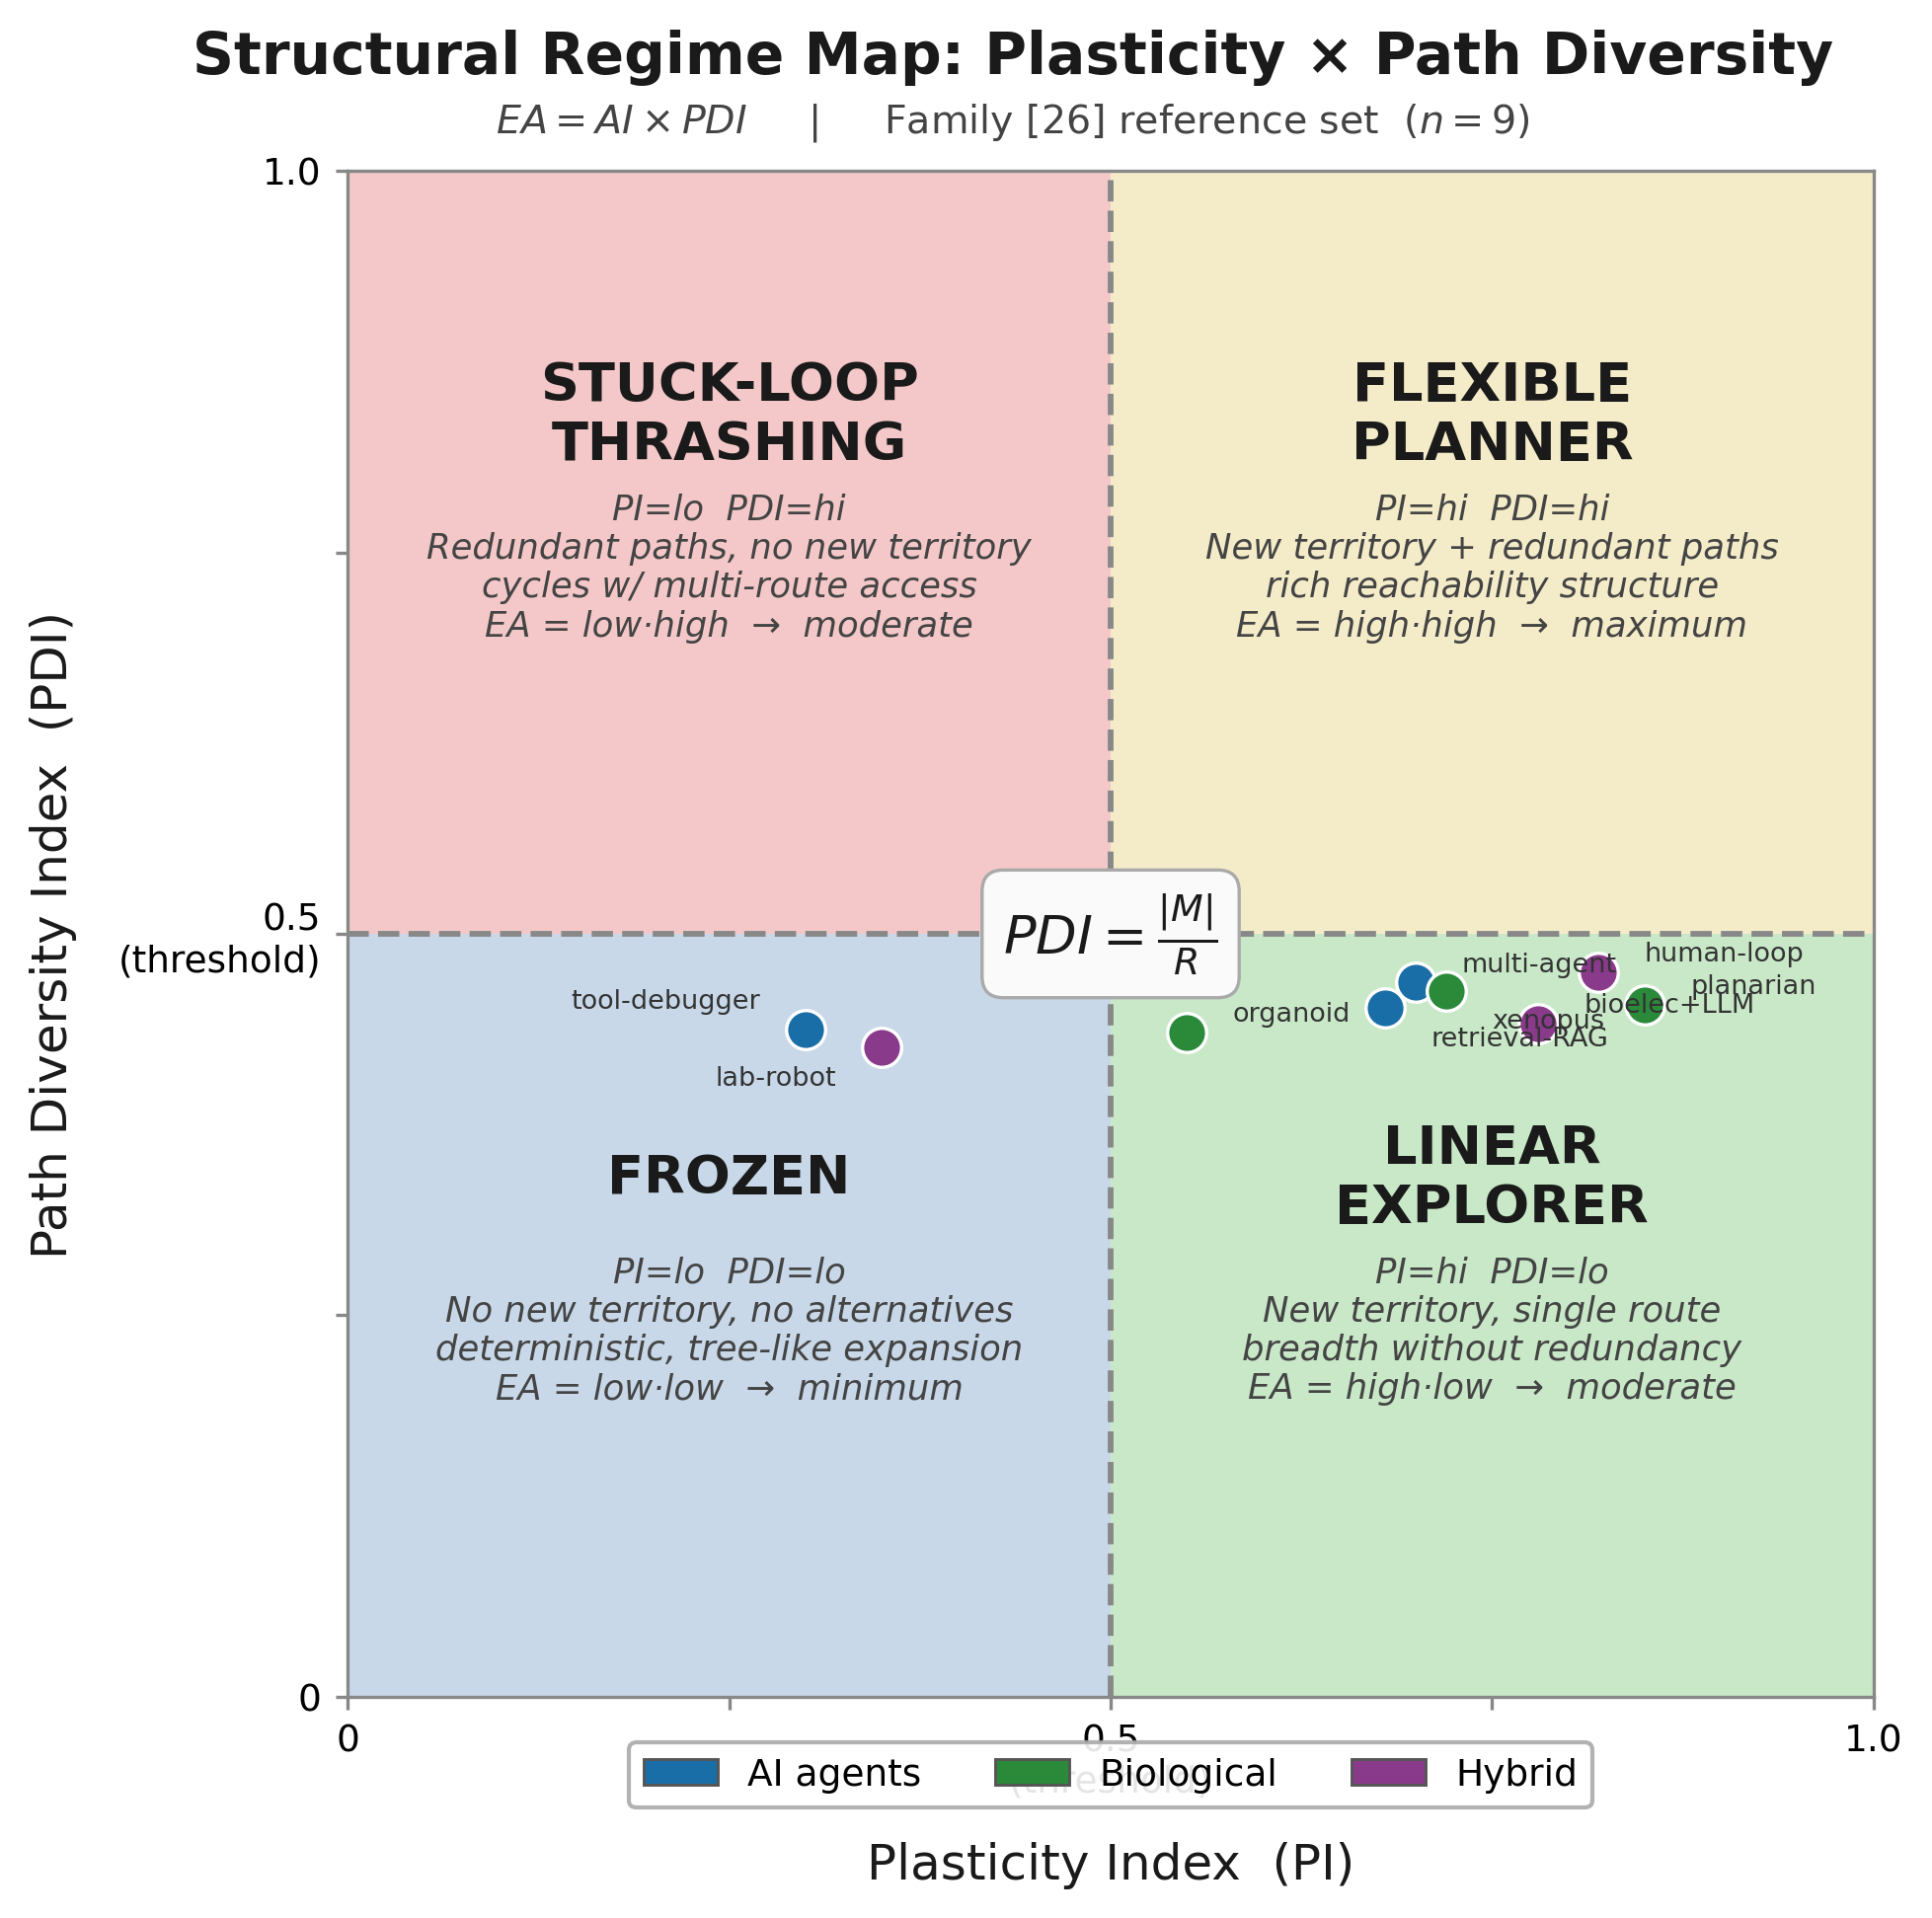
\includegraphics[width=0.72\textwidth]{pi_pdi_quadrant.png}
  \caption{%
    \textbf{Structural regime map} with nine synthetic reference
    exemplars ($n=9$, Table~\ref{tab:refset}).
    All nine fall below $\PDI = 0.5$
    (range $0.425$--$0.475$), clustering in the \emph{Linear Explorer}
    regime ($n=7$) or \emph{Frozen} ($n=2$).
    No exemplar reaches \emph{Flexible Planner} or \emph{Stuck-Loop
    Thrashing}.}
  \label{fig:regimes}
\end{figure}

% ─────────────────────────────────────────────────────────────────────────────
\section{PDI--Obstruction Bridge}
\label{sec:bridge}

\paragraph{Failure algebra.}
The QA Failure Algebra \cite{QAFamily76Cert,QAFamily86Cert} defines a
bounded join-semilattice over failure modes
$\carrier = \{\OK, \PB, \IV, \OD\}$ with partial order
$\OK < \PB, \IV < \OD$ (strict, forming a diamond lattice with $\OK$ as
bottom and $\OD$ as top).
The join operation satisfies: $\OK \jn \OK = \OK$,
$\OK \jn \PB = \PB$, $\PB \jn \IV = \OD$, etc.
Each generator $g$ receives a failure tag $\tau(g) \in \carrier$
denoting its worst-case failure mode.

\paragraph{Obstruction types.}
Let $O \subseteq E$ be a named obstruction (a set of generator edges
conditionally blocked) and $G_O = (V, E \setminus O)$
the residual graph. Write $R_O = R(G_O)$, $M_O = M(G_O)$.

\begin{definition}[Obstruction types]
  \begin{itemize}
    \item \textbf{Type I} (state-annihilating): $R_O \subsetneq R$.
    \item \textbf{Type II} (route-reducing): $R_O = R$,
      $M_O \subsetneq M$; $\PDI$ strictly decreases.
    \item \textbf{Type III} (topology-preserving): $R_O = R$, $M_O = M$;
      $\PDI$ unchanged.
  \end{itemize}
  These three cases are exhaustive and mutually exclusive.
\end{definition}

\begin{theorem}[Failure-Tag Obstruction Typing]
  \label{thm:bridge}
  \begin{itemize}
    \item $\tau(g) = \OK$ $\Rightarrow$ $g$'s edges are never blocked,
      so $O_g = \emptyset$ (Type~III vacuously).
    \item $\tau(g) \in \{\PB, \IV\}$ $\Rightarrow$ $O_g$ is Type~I if
      blocking $g$'s edges removes states from $R$; Type~II if
      $R$ is preserved but merge edges for some states in $M$ are lost.
    \item $\tau(g) = \OD$ $\Rightarrow$ $g$'s edges are permanently absent;
      if any state $v \in R$ is reachable only through $g$, then
      $v \notin R_O$ (Type~I).
  \end{itemize}
\end{theorem}

\begin{corollary}[Merge Stability Criterion]
  \label{cor:merge}
  A sufficient condition for $\PDI(G) > 0.5$ is:
  there exists a set $S \subseteq R$ with $|S| > |R|/2$ such that
  every $v \in S$ is reachable via $\geq 2$ distinct paths in $\Ghat$
  provided by generator sequences whose merging edges use only generators
  $g_1, g_2$ satisfying $\tau(g_1) \jn \tau(g_2) = \OK$.
  Any merge-path pair with $\tau(g_1) \jn \tau(g_2) \geq \PB$
  risks simultaneous blocking, collapsing $v$ to a single route
  (Type~II obstruction on $S$).
\end{corollary}

\paragraph{Reference set obstruction analysis.}
Of the 16 named obstructions across the nine reference exemplars,
8 are Type~I (state-annihilating: \texttt{context\_overflow},
\texttt{consensus\_deadlock}, \texttt{energy\_exhaustion}, etc.)
and 9 are Type~II (route-reducing: \texttt{message\_loss},
\texttt{electrode\_drift}, \texttt{tip\_clog}, etc.).
Zero Type~III obstructions appear in the reference set.

% ─────────────────────────────────────────────────────────────────────────────
\section{Experiments}
\label{sec:experiments}

\subsection{Reference Exemplar Survey}
\label{sec:baseline}

Nine synthetic exemplars were constructed under the QA Competency
Detection Framework \cite{QAFamily26Cert} to represent three substrate
domains at differing competency levels.
These are hand-crafted illustrative certs, not measurements from
specific wet-lab or deployed systems.
Table~\ref{tab:refset} gives the per-exemplar metrics.

\begin{table}[h]
  \centering
  \small
  \begin{tabular}{llcccc}
    \toprule
    System & Domain & $\AI$ & $\PI$ & $\PDI$ & Regime \\
    \midrule
    multi\_agent\_coord.   & AI     & 0.750 & 0.700 & 0.468 & Lin.\ Expl. \\
    retrieval\_arag        & AI     & 0.820 & 0.680 & 0.451 & Lin.\ Expl. \\
    tool\_debugger         & AI     & 0.640 & 0.300 & 0.438 & Frozen      \\
    organoid\_self\_repair & Bio    & 0.620 & 0.550 & 0.436 & Lin.\ Expl. \\
    planarian\_regen       & Bio    & 0.710 & 0.850 & 0.454 & Lin.\ Expl. \\
    xenopus\_patterning    & Bio    & 0.880 & 0.720 & 0.463 & Lin.\ Expl. \\
    bioelectric\_llm       & Hybrid & 0.680 & 0.780 & 0.441 & Lin.\ Expl. \\
    human\_in\_the\_loop   & Hybrid & 0.910 & 0.820 & 0.475 & Lin.\ Expl. \\
    lab\_robot             & Hybrid & 0.550 & 0.350 & 0.425 & Frozen      \\
    \bottomrule
  \end{tabular}
  \caption{Per-exemplar competency metrics.
    $\PDI$ range $0.425$--$0.475$ across all nine; 7/9 in
    \emph{Linear Explorer}, 2/9 in \emph{Frozen}.
    Bio systems show higher mean $\PI$ (0.71) vs.\ AI (0.56)
    while $\PDI$ is compressed across domains (range $< 0.05$).}
  \label{tab:refset}
\end{table}

The compressed $\PDI$ band is structurally expected.
All nine exemplars have branching-factor-bounded generator graphs
constructed without deliberate merge engineering.
By Proposition~\ref{prop:grid_pdi}, achieving $\PDI > 0.5$ requires
either $A \geq 3, D \geq 3$ in an idealised grid, or equivalent
fan-then-merge topology --- absent from the reference construction protocol.

\subsection{Synthetic Existence Proof}
\label{sec:existence}

\paragraph{Construction.}
We instantiate $G_{4,6}$ (Proposition~\ref{prop:grid_pdi}):
apex $s_0$; generators $\texttt{adv}_k$ and $\texttt{cl}_k$ for $k=0,\ldots,3$;
all $\tau = \OK$.
$|R| = 25$, $|M| = 20$.

\paragraph{Closed-form verification.}
By Proposition~\ref{prop:grid_pdi} with $A=4$, $D=6$:
\[
  \PDI = \frac{4 \times 5}{1 + 24} = \frac{20}{25} = 0.800,
  \quad \PI = 0.750, \quad \EA = 0.625 \times 0.800 = 0.500.
\]
All generators $\tau = \OK$; by Corollary~\ref{cor:merge},
$\tau(g_1) \jn \tau(g_2) = \OK$ for all merge pairs,
so all obstructions are vacuously Type~III.
\textbf{Regime: \emph{Flexible Planner} ($\PI > 0.5$, $\PDI > 0.5$).}
This is the first constructive existence proof that the upper-right
quadrant of Figure~\ref{fig:regimes} is non-empty.

\subsection{Controlled Obstruction Perturbation}
\label{sec:perturbation}

\paragraph{Protocol.}
Starting from $G_{4,6}$, we promote $k$ generators
$\{\texttt{cl}_i\}_{i < k}$ from $\tau=\OK$ to $\tau=\PB$
(permanently blocked), for $k = 0,1,2,3,4$.

\paragraph{Closed-form result.}
Blocking $\texttt{cl}_j$ removes the unique merge path to
$\mathrm{arm}_{(j+1)\%4,d}$ for $d \geq 2$: those five states exit $M$
(Type~II obstruction on $\mathrm{arm}_{(j+1)\%4}$) while remaining in $R$.
Arms are independent, so effects do not compound across arms.
By Proposition~\ref{prop:grid_pdi} applied to the residual graph
(now $A - k$ arms retain merge edges):
\[
  \PDI(k) = \frac{(4-k) \cdot 5}{25} = 0.800 - 0.200\,k,
  \quad \EA(k) = 0.625 \times \PDI(k) = 0.500 - 0.125\,k.
\]
\paragraph{Regime collapse.}
At $k = 2$: $\PDI = 0.400 < 0.5$.
The system transitions from \emph{Flexible Planner} to
\emph{Linear Explorer}; $\EA$ halves from $0.500$ to $0.250$.
At $k=4$: $\PDI = 0$, regime is \emph{Frozen}.
Two certified bundles (\texttt{1block}: $\PDI=0.600$;
\texttt{2block}: $\PDI=0.400$) validate the formula.
Figure~\ref{fig:fragility} depicts the full sweep.

\begin{figure}[t]
  \centering
  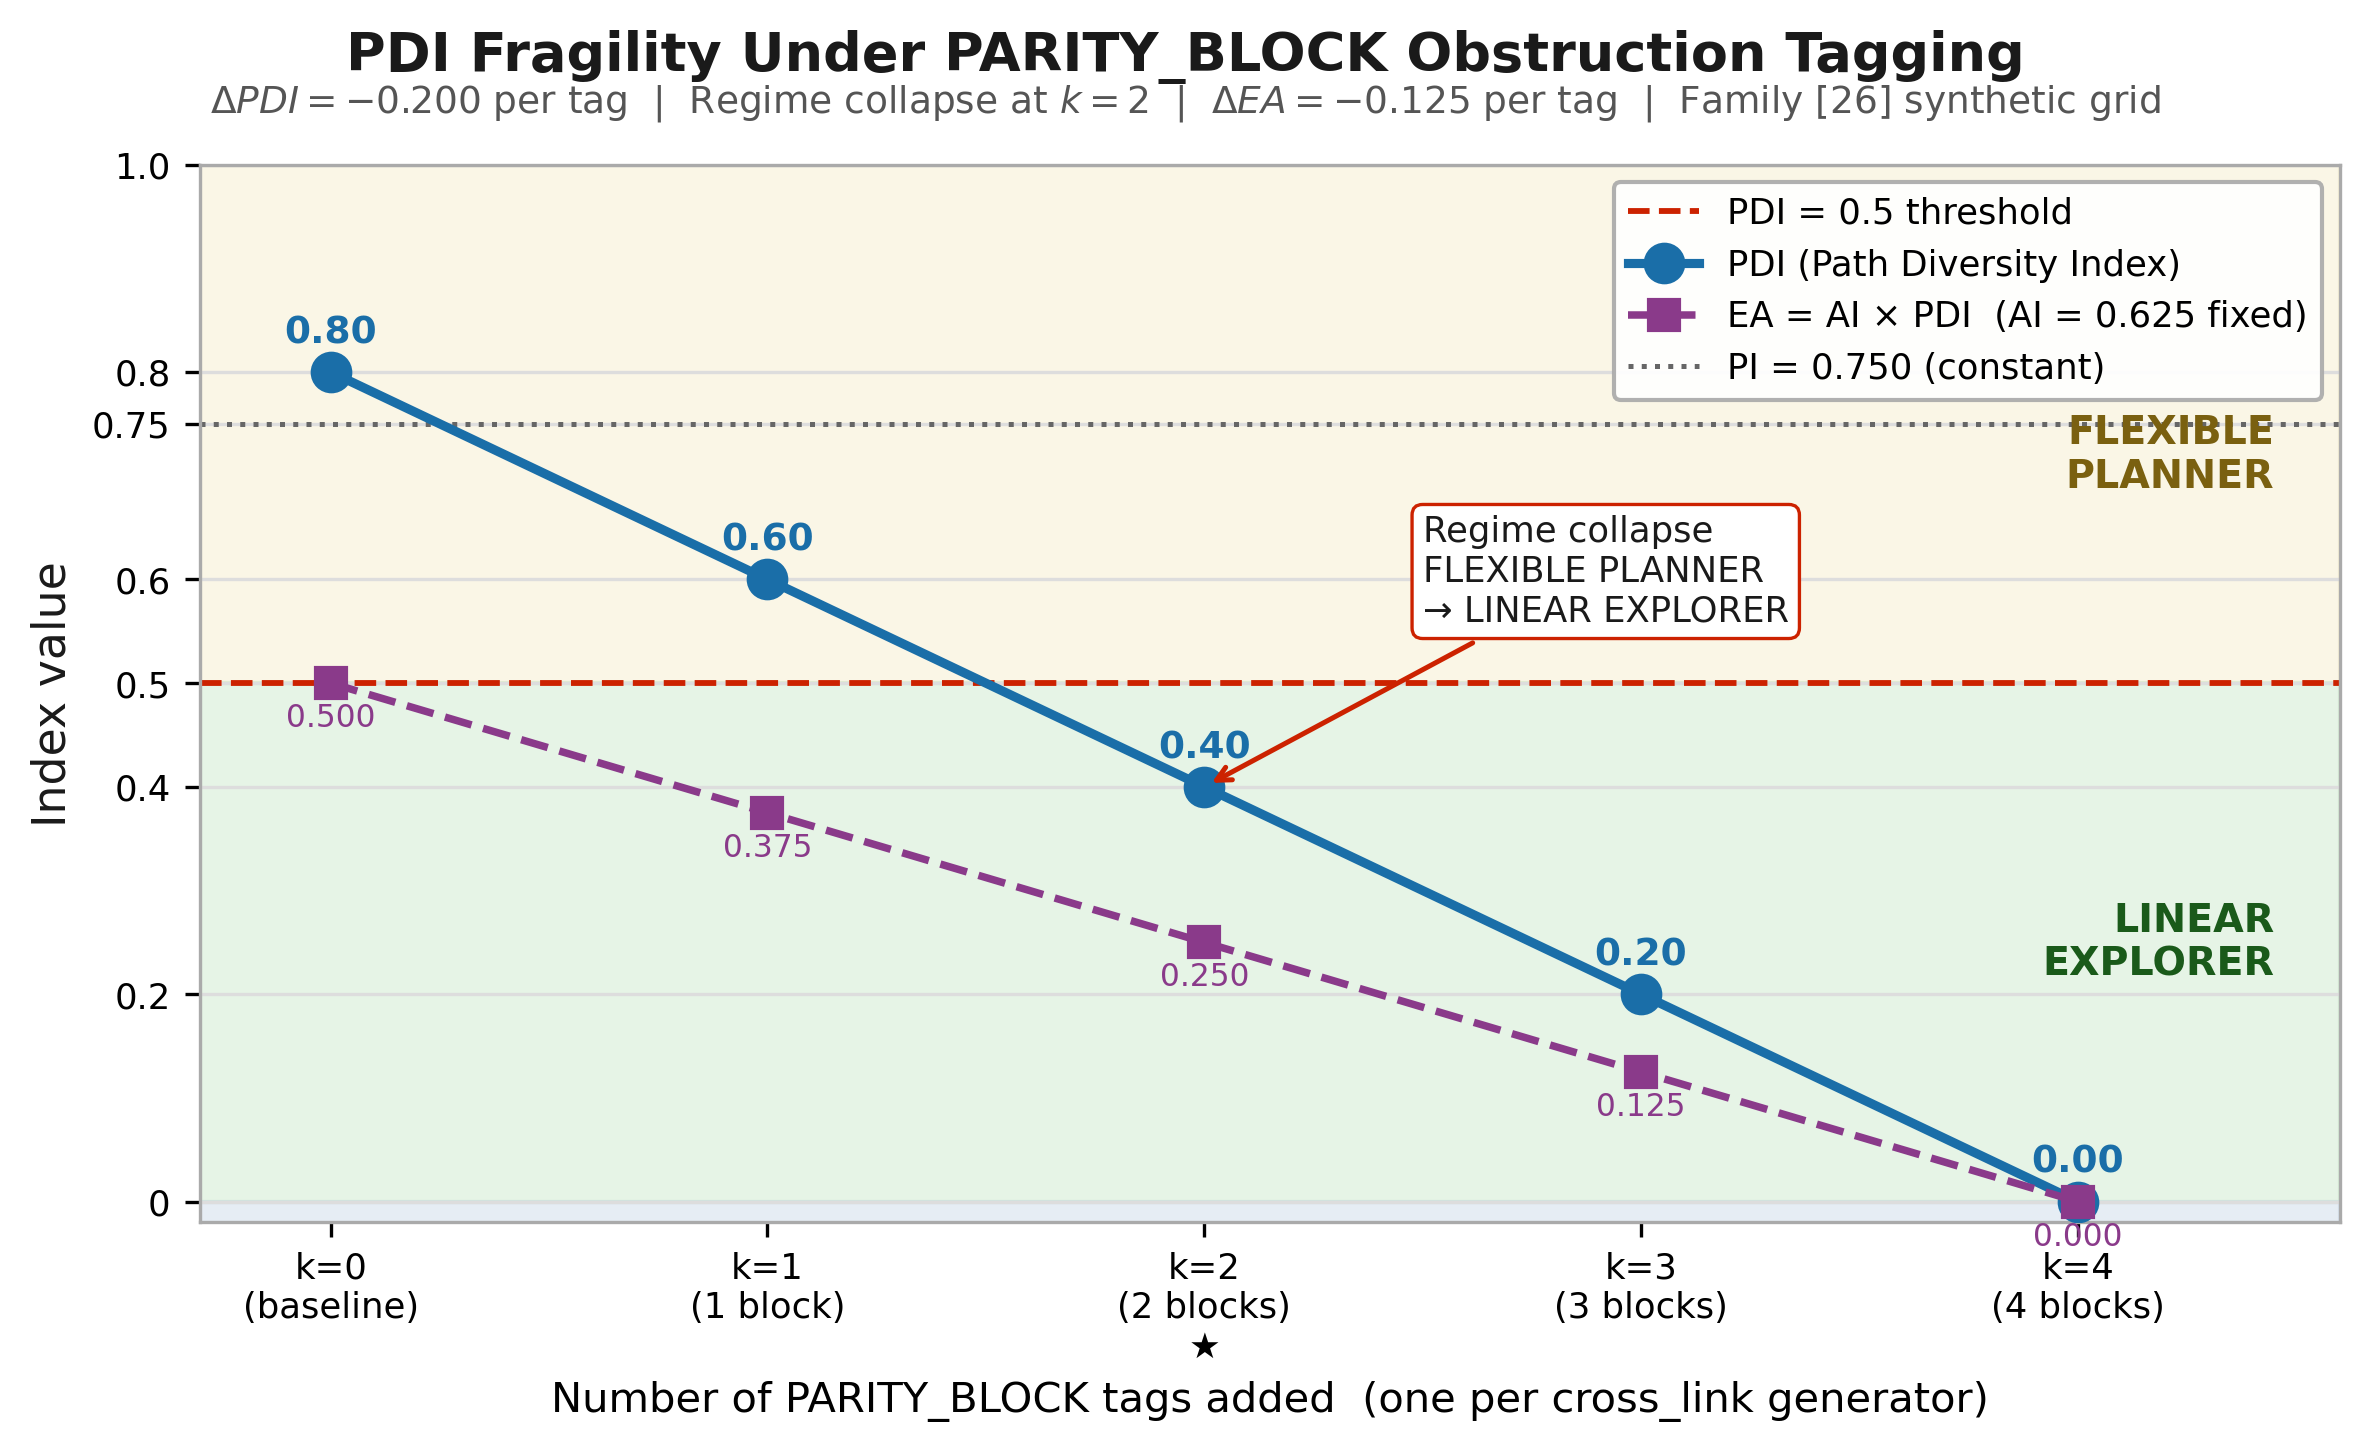
\includegraphics[width=0.82\textwidth]{pi_pdi_fragility.png}
  \caption{%
    \textbf{PDI fragility} under \PB{} tagging.
    $\PDI$ (solid blue) and $\EA$ (dashed purple) versus $k$
    (number of blocked cross-link generators).
    The formula $\PDI(k) = 0.800 - 0.200k$ holds exactly for $G_{4,6}$.
    Regime collapse (dashed red: $\PDI = 0.5$) occurs at $k=2$ (star).
    $\PI = 0.750$ (dotted) is constant throughout.
    The linear drop is a property of the symmetric cyclic construction;
    asymmetric generator graphs will show a non-linear response.}
  \label{fig:fragility}
\end{figure}

% ─────────────────────────────────────────────────────────────────────────────
\section{Discussion}
\label{sec:discussion}

\paragraph{PDI is not captured by existing metrics.}
$\AI$ measures how much of the state space is reachable;
$\PI$ measures how quickly that reach changes under perturbation.
Neither asks whether the reachable region is accessible via multiple
independent routes.
A system can have high $\AI$ and high $\PI$
yet be entirely brittle under a single generator failure
($\PDI = 0$ means every reachable state has exactly one path;
one blocked generator can strand arbitrary state subsets).
$\PDI$ is independently necessary for $\EA$-maximising design.

\paragraph{The Merge Stability Criterion is a design target.}
Corollary~\ref{cor:merge} translates $\PDI > 0.5$ into a concrete
engineering requirement:
more than half of reachable states must have $\geq 2$ merge paths
via $\OK$-tagged generators.
Generator count alone is insufficient;
\emph{merge topology} --- reconvergent paths in the condensation DAG ---
is the decisive structural factor.
The synthetic experiment quantifies the cost: two blocked generators
suffice to collapse $\PDI$ below $0.5$ in the $G_{4,6}$ construction.

\paragraph{Certification chain.}
The obstruction bridge (\S\ref{sec:bridge}) closes a three-family
certification chain:
\[
  \text{Family [76] failure algebra}
  \;\xrightarrow{\text{tagging [86]}}\;
  \text{T2/T3 SCC bounds}
  \;\xrightarrow{\text{Theorem~\ref{thm:bridge}}}\;
  \PDI
  \;\xrightarrow{\text{Definition~\ref{def:ea}}}\;
  \EA.
\]
$\PDI$ is derivable from the T3 path-propagation witness without
additional BFS computation.

\paragraph{Limitations.}
(i)~The five competency metrics are defined over generator graphs;
continuous state spaces require discretisation and $\PDI$ will depend
on resolution.
(ii)~The $0.5$ regime thresholds are operational, not phase-transition-derived;
their justification is left to future work.
(iii)~The reference exemplars are synthetic hand-crafted certs;
$\PDI$ measurements on real biological or deployed AI systems require
empirical generator-graph reconstruction.
(iv)~The linear $\PDI$ collapse ($-0.200$ per tag) is specific to the
symmetric $G_{4,6}$ construction; asymmetric graphs will exhibit
non-linear responses.

% ─────────────────────────────────────────────────────────────────────────────
\section{Conclusion}

We have defined $\PDI$, proved the SCC Saturation Lemma,
No Artificial Inflation Theorem, Cyclic Grid Proposition, and Cyclic Thrashing
Theorem, introduced Effective Agency $\EA = \AI \times \PDI$ as a product
metric, connected $\PDI$ to the failure algebra via the PDI--Obstruction Bridge,
and provided both a constructive existence proof ($\PDI = 0.800$)
and a fragility experiment ($\PDI(k) = 0.800 - 0.200k$, collapse at $k=2$).

The central message:
\begin{quote}
  Flexible planning is not accidental.
  It requires merge topology with obstruction joins $= \OK$.
  In the symmetric $G_{4,6}$ construction, two blocked generators
  suffice to eliminate it.
\end{quote}

All certified artefacts, figure generators, and reference bundles are
available at tag \texttt{family-26-figure2-fragility-v1.0.0}
\cite{QAFamily26Cert}.

% ─────────────────────────────────────────────────────────────────────────────
\bibliographystyle{plainnat}
\bibliography{refs}

\end{document}
